% Options for packages loaded elsewhere
\PassOptionsToPackage{unicode}{hyperref}
\PassOptionsToPackage{hyphens}{url}
\PassOptionsToPackage{dvipsnames,svgnames,x11names}{xcolor}
\documentclass[
  english,
  10pt,
]{article}
\usepackage{xcolor}
\usepackage[margin=0.85in]{geometry}
\usepackage{amsmath,amssymb}
\setcounter{secnumdepth}{-\maxdimen} % remove section numbering
\usepackage{iftex}
\ifPDFTeX
  \usepackage[T1]{fontenc}
  \usepackage[utf8]{inputenc}
  \usepackage{textcomp} % provide euro and other symbols
\else % if luatex or xetex
  \usepackage{unicode-math} % this also loads fontspec
  \defaultfontfeatures{Scale=MatchLowercase}
  \defaultfontfeatures[\rmfamily]{Ligatures=TeX,Scale=1}
\fi
\usepackage{lmodern}
\ifPDFTeX\else
  % xetex/luatex font selection
  \setmainfont[]{DejaVu Serif}
  \setsansfont[]{DejaVu Sans}
  \setmonofont[]{DejaVu Sans Mono}
\fi
% Use upquote if available, for straight quotes in verbatim environments
\IfFileExists{upquote.sty}{\usepackage{upquote}}{}
\IfFileExists{microtype.sty}{% use microtype if available
  \usepackage[]{microtype}
  \UseMicrotypeSet[protrusion]{basicmath} % disable protrusion for tt fonts
}{}
\usepackage{setspace}
\makeatletter
\@ifundefined{KOMAClassName}{% if non-KOMA class
  \IfFileExists{parskip.sty}{%
    \usepackage{parskip}
  }{% else
    \setlength{\parindent}{0pt}
    \setlength{\parskip}{6pt plus 2pt minus 1pt}}
}{% if KOMA class
  \KOMAoptions{parskip=half}}
\makeatother
\usepackage{color}
\usepackage{fancyvrb}
\newcommand{\VerbBar}{|}
\newcommand{\VERB}{\Verb[commandchars=\\\{\}]}
\DefineVerbatimEnvironment{Highlighting}{Verbatim}{commandchars=\\\{\}}
% Add ',fontsize=\small' for more characters per line
\newenvironment{Shaded}{}{}
\newcommand{\AlertTok}[1]{\textcolor[rgb]{1.00,0.00,0.00}{\textbf{#1}}}
\newcommand{\AnnotationTok}[1]{\textcolor[rgb]{0.38,0.63,0.69}{\textbf{\textit{#1}}}}
\newcommand{\AttributeTok}[1]{\textcolor[rgb]{0.49,0.56,0.16}{#1}}
\newcommand{\BaseNTok}[1]{\textcolor[rgb]{0.25,0.63,0.44}{#1}}
\newcommand{\BuiltInTok}[1]{\textcolor[rgb]{0.00,0.50,0.00}{#1}}
\newcommand{\CharTok}[1]{\textcolor[rgb]{0.25,0.44,0.63}{#1}}
\newcommand{\CommentTok}[1]{\textcolor[rgb]{0.38,0.63,0.69}{\textit{#1}}}
\newcommand{\CommentVarTok}[1]{\textcolor[rgb]{0.38,0.63,0.69}{\textbf{\textit{#1}}}}
\newcommand{\ConstantTok}[1]{\textcolor[rgb]{0.53,0.00,0.00}{#1}}
\newcommand{\ControlFlowTok}[1]{\textcolor[rgb]{0.00,0.44,0.13}{\textbf{#1}}}
\newcommand{\DataTypeTok}[1]{\textcolor[rgb]{0.56,0.13,0.00}{#1}}
\newcommand{\DecValTok}[1]{\textcolor[rgb]{0.25,0.63,0.44}{#1}}
\newcommand{\DocumentationTok}[1]{\textcolor[rgb]{0.73,0.13,0.13}{\textit{#1}}}
\newcommand{\ErrorTok}[1]{\textcolor[rgb]{1.00,0.00,0.00}{\textbf{#1}}}
\newcommand{\ExtensionTok}[1]{#1}
\newcommand{\FloatTok}[1]{\textcolor[rgb]{0.25,0.63,0.44}{#1}}
\newcommand{\FunctionTok}[1]{\textcolor[rgb]{0.02,0.16,0.49}{#1}}
\newcommand{\ImportTok}[1]{\textcolor[rgb]{0.00,0.50,0.00}{\textbf{#1}}}
\newcommand{\InformationTok}[1]{\textcolor[rgb]{0.38,0.63,0.69}{\textbf{\textit{#1}}}}
\newcommand{\KeywordTok}[1]{\textcolor[rgb]{0.00,0.44,0.13}{\textbf{#1}}}
\newcommand{\NormalTok}[1]{#1}
\newcommand{\OperatorTok}[1]{\textcolor[rgb]{0.40,0.40,0.40}{#1}}
\newcommand{\OtherTok}[1]{\textcolor[rgb]{0.00,0.44,0.13}{#1}}
\newcommand{\PreprocessorTok}[1]{\textcolor[rgb]{0.74,0.48,0.00}{#1}}
\newcommand{\RegionMarkerTok}[1]{#1}
\newcommand{\SpecialCharTok}[1]{\textcolor[rgb]{0.25,0.44,0.63}{#1}}
\newcommand{\SpecialStringTok}[1]{\textcolor[rgb]{0.73,0.40,0.53}{#1}}
\newcommand{\StringTok}[1]{\textcolor[rgb]{0.25,0.44,0.63}{#1}}
\newcommand{\VariableTok}[1]{\textcolor[rgb]{0.10,0.09,0.49}{#1}}
\newcommand{\VerbatimStringTok}[1]{\textcolor[rgb]{0.25,0.44,0.63}{#1}}
\newcommand{\WarningTok}[1]{\textcolor[rgb]{0.38,0.63,0.69}{\textbf{\textit{#1}}}}
\usepackage{longtable,booktabs,array}
\usepackage{calc} % for calculating minipage widths
% Correct order of tables after \paragraph or \subparagraph
\usepackage{etoolbox}
\makeatletter
\patchcmd\longtable{\par}{\if@noskipsec\mbox{}\fi\par}{}{}
\makeatother
% Allow footnotes in longtable head/foot
\IfFileExists{footnotehyper.sty}{\usepackage{footnotehyper}}{\usepackage{footnote}}
\makesavenoteenv{longtable}
\usepackage{graphicx}
\makeatletter
\newsavebox\pandoc@box
\newcommand*\pandocbounded[1]{% scales image to fit in text height/width
  \sbox\pandoc@box{#1}%
  \Gscale@div\@tempa{\textheight}{\dimexpr\ht\pandoc@box+\dp\pandoc@box\relax}%
  \Gscale@div\@tempb{\linewidth}{\wd\pandoc@box}%
  \ifdim\@tempb\p@<\@tempa\p@\let\@tempa\@tempb\fi% select the smaller of both
  \ifdim\@tempa\p@<\p@\scalebox{\@tempa}{\usebox\pandoc@box}%
  \else\usebox{\pandoc@box}%
  \fi%
}
% Set default figure placement to htbp
\def\fps@figure{htbp}
\makeatother
\ifLuaTeX
\usepackage[bidi=basic,shorthands=off,]{babel}
\else
\usepackage[bidi=default,shorthands=off,]{babel}
\fi
\ifPDFTeX
\else
\babelfont{rm}[]{DejaVu Serif}
\fi
\ifLuaTeX
  \usepackage{selnolig} % disable illegal ligatures
\fi
\setlength{\emergencystretch}{3em} % prevent overfull lines
\providecommand{\tightlist}{%
  \setlength{\itemsep}{0pt}\setlength{\parskip}{0pt}}
\usepackage{xurl}
\usepackage{needspace}
\urlstyle{tt}
\setlength{\emergencystretch}{3em}
\usepackage{fvextra}
\DefineVerbatimEnvironment{verbatim}{Verbatim}{breaklines=true,fontsize=\small}
\usepackage{fancyhdr}
\pagestyle{fancy}
\fancyhf{}
\fancyhead[L]{\small LeasePath --- Working draft v1}
\fancyhead[R]{\small November 10, 2026}
\fancyfoot[C]{\thepage}
\setlength{\headheight}{14pt}
\usepackage{bookmark}
\IfFileExists{xurl.sty}{\usepackage{xurl}}{} % add URL line breaks if available
\urlstyle{same}
\hypersetup{
  pdftitle={LeasePath: Distribution-Aware KV Cache Retention for Tool-Augmented LLM Agents},
  pdfauthor={Working draft v1 --- author information to be added},
  pdflang={en},
  colorlinks=true,
  linkcolor={blue},
  filecolor={Maroon},
  citecolor={Blue},
  urlcolor={blue},
  pdfcreator={LaTeX via pandoc}}

\title{LeasePath: Distribution-Aware KV Cache Retention for
Tool-Augmented LLM Agents}
\author{Working draft v1 --- author information to be added}
\date{November 10, 2026}

\begin{document}
\maketitle

\setstretch{1.03}
\textbf{Draft status.} This manuscript develops the November 10 outline
into a complete first draft. Performance claims refer exclusively to the
completed development experiments described below. The independent
evaluation and pressure matrix are not reported as completed. The PDF
uses a reading layout, not an official conference template. Local
evidence is indexed in Appendix G; the companion Chinese revision notes
identify remaining work.

\section{Abstract}\label{abstract}

Tool-augmented large language model agents alternate between model
execution and external computation, creating uncertain intervals before
compatible key--value (KV) prefixes are needed again. Predicting tool
completion or increasing cache hits does not necessarily reduce task
completion time. We study how a distribution of the time to the next
legal prefix demand can guide KV retention. LeasePath distinguishes
demand from explicit relationship retirement and observation censoring,
and converts cumulative demand probabilities into a finite-horizon
discounted retention score. A pressure-triggered eviction procedure
applies this score subject to active-reference protection, prefix
dependencies, and shared physical occupancy. We implement the policy in
a native inference backend and audit consumed tool feedback, actual KV
actions, executed prefill, and final-answer validation. In a preliminary
shared-server experiment with three known development tasks,
distribution scoring with equal cost multipliers reuses 768 additional
tokens per three-session batch, reduces aggregate prefill time by
14.600\%, and reduces mean task completion time by 2.929\% relative to
retired-first LRU. Using the same frozen predictor, it reduces mean
completion time by 1.723\% relative to a three-second
cumulative-probability score. A calibrated cost multiplier provides no
additional benefit, and conditional empirical distributions outperform
the frozen boosted-tree predictor offline. These observations support
the feasibility of the decision mechanism in this workload; its value on
independent task families and against complete prior systems remains
unestablished.

\section{1 Introduction}\label{introduction}

An LLM agent often pauses model execution to run a tool, inspect its
result, and continue generation with an extended conversation. The KV
state of the preceding context can save substantial prefill work when
that conversation resumes. During the pause, however, the state occupies
capacity that other sessions could use. Retaining every idle prefix is
infeasible under pressure, while immediately discarding it can turn a
later continuation into redundant computation. The useful question is
therefore whether an idle prefix will be needed again, when that demand
will occur, and which physically feasible retention choice is worth its
capacity.

Recency captures when a prefix was last used, but it does not directly
describe progress through external computation. A tool that has been
running for several seconds may be close to completion or may still have
a long remaining duration. Workflow step distance also need not
correspond to elapsed time: one step can be a short lookup or a long
numerical computation. Even when the next-use time can be estimated, a
single scalar need not preserve all information relevant to retention.
Two prefixes can have the same probability of demand within a short
window yet assign the remaining demand probability to very different
times.

Prior work already uses tool durations, elapsed-time conditioning,
empirical distributions, workflow structure, and termination
probabilities to manage agent KV caches. In particular, CacheWise
estimates remaining tool time, Continuum selects time-to-live values
from distributions, and PBKV uses discounted probabilistic lookahead
over future invocations. LeasePath does not claim these ideas
individually. We investigate a more specific connection: a distribution
over \textbf{wall-clock time to the next legal prefix demand}, evaluated
at a causal decision snapshot, can be mapped to a retention score and
applied to the currently feasible physical eviction actions. The
resulting hypothesis is testable with a fixed predictor: preserving
timing information across a common horizon may change which useful
prefixes survive compared with evaluating the same distribution at one
time threshold.

Three issues make that hypothesis nontrivial. First, the prediction
target must correspond to demand. Tool completion, request readiness,
and cache lookup are separate events. A lookup that misses still
establishes demand, while an observation window ending does not
establish that reuse will never occur. Second, scores act on a
constrained cache. Active references cannot be evicted, a retained
descendant requires its prefix, and several owners can share one
physical block. Third, avoided prefill is only one component of
completion time. Tool variation, queueing, generation differences, and
controller overhead can offset a cache improvement.

LeasePath addresses these issues through a demand-based event
definition, a finite-horizon discounted score, and a controller that
repeatedly chooses legal leaves of the resident prefix structure. The
score integrates unconditional demand probability mass; it neither
conditions on eventual reuse nor reallocates unresolved tail mass into
the supported window. The main configuration gives all candidates the
same recomputation-cost multiplier, allowing the
distribution-to-decision mapping to be examined separately from an
estimated cost model.

The present evidence is deliberately limited to a completed prototype
and development experiments. On three known tasks, equal-cost
distribution scoring improves observed reuse, aggregate prefill time,
and mean submission-to-validated-answer time relative to two internal
baselines. The results also expose two limitations: a more complex
predictor is less accurate than conditional empirical estimation on the
current data, and adding a separately calibrated marginal-cost
multiplier worsens the observed result. These findings make predictor
choice, score choice, and end-to-end benefit distinct empirical
questions.

This draft makes three contributions within that scope:

\begin{enumerate}
\def\labelenumi{\arabic{enumi}.}
\tightlist
\item
  A prediction and measurement formulation that separates the first
  legal KV demand, explicit retirement of an owner--context
  relationship, and observation censoring, while keeping physical hit
  outcomes out of demand labels.
\item
  An implemented mapping from finite-horizon demand distributions to
  legal, pressure-triggered KV eviction, with explicit treatment of
  prefix dependencies, shared ownership, support failure, and
  deterministic tie-breaking.
\item
  An audited preliminary evaluation that measures actual prefill and
  validated-answer completion time, alongside predictor comparisons and
  a negative result for the cost extension.
\end{enumerate}

These contributions establish an implementation and an initial empirical
case. They do not establish superiority to CacheWise or Continuum, broad
generalization, or optimal cache control.

\section{2 Background and Related
Work}\label{background-and-related-work}

\subsection{2.1 Agent execution and prefix
reuse}\label{agent-execution-and-prefix-reuse}

During prefill, a transformer constructs KV state for input tokens;
during decoding, it extends the state as it generates output. A
compatible cached token prefix can reduce the input portion that must be
processed again. Compatibility depends on the actual tokens and the
model, tokenizer, position treatment, and KV configuration. Similar text
or a shared task identifier is insufficient.

When a model call finishes, its context may become idle while an
external tool runs. A subsequent request typically appends tool feedback
and protocol text. The tool can finish before the client constructs this
request, and a ready request can wait before the backend performs its
lookup. For a simple serial dependency, the remaining time to lookup can
be decomposed as

\[
R_{\mathrm{lookup}}=R_{\mathrm{tool}}+D_{\mathrm{client}}
 +W_{\mathrm{queue}}+D_{\mathrm{dispatch\to lookup}}.
\]

For parallel tools or branches, dependency completion replaces the
single-tool term. This decomposition explains why tool duration is an
imperfect label for cache demand; it does not imply that all components
are observable to the current predictor. Our frozen predictor has no
measured queue-state feature.

Our prototype runs concurrent agent sessions and tools, while serving
model requests serially in first-come, first-served (FCFS) order.
Changing retention can change service time, subsequent tool launches,
and later arrivals. Consequently, replaying a fixed baseline lookup
timeline is useful for diagnosing decisions but cannot reproduce another
policy's natural completion time.

\subsection{2.2 Time-aware KV
management}\label{time-aware-kv-management}

InferCept estimates interception duration to choose among preservation,
recomputation, and swapping (Abhyankar et al., 2024). Continuum uses
empirical tool-duration distributions to choose KV time-to-live values,
incorporating prefill or reload costs and queueing effects, and combines
retention with program-level scheduling (Li et al., 2025, version 7).
CacheWise clusters tool arguments using TF-IDF and KMeans, conditions
historical duration distributions on elapsed waiting time, and ranks
candidates using estimated next-use time (Tiwari et al., 2026).

These systems establish direct precedents for using distributions, tool
metadata, and elapsed time. Our controlled question concerns the
decision functional applied to a common prediction: a fixed-window
demand probability versus discounted mass across a finite horizon, under
the same prefix constraints. The fixed-window baseline in this draft is
\(F_U(3\,\mathrm{s})\). It is a cumulative probability, not a point
estimate of return time and not an implementation of CacheWise.
Complete-system comparisons must additionally account for scheduling,
prediction features, and available storage tiers.

\subsection{2.3 Workflow structure, lifecycle, and
sharing}\label{workflow-structure-lifecycle-and-sharing}

KVFlow uses an Agent Step Graph and steps-to-execution to prioritize
shared prefix nodes (Pan et al., 2025). Its dependencies include both
all-predecessor and alternative-predecessor conditions, and its full
system includes prefetching and scheduling. PBKV predicts future agent
invocations from workflow history, graph structure, and prefill
representations (Zheng et al., 2026). Its multistep score already
combines termination probabilities, survival across steps, confidence
discounting, and aggregation across workflows. LeasePath therefore does
not present probabilistic lookahead, termination-aware scoring, or
discounting as new in themselves. Its target is a first compatible
demand in wall-clock time, and its implementation evaluates that target
through legal prefix eviction.

Lifecycle information is also an important baseline. KVTether maps
message lifecycle information to KV states, reclaims dead state first,
and applies MRU among live-but-idle entries to exploit delayed reuse (Fu
et al., 2026). PBKV likewise prioritizes entries whose associated
workflows have terminated. Any claimed gain from distribution
information must be separated from reclaiming already retired state. We
therefore use retired-first LRU as an internal comparator; this does not
reproduce the full KVTether policy.

\subsection{2.4 Learned prediction and competing
risks}\label{learned-prediction-and-competing-risks}

Prediction-guided caching has a broader history, including Learning
Relaxed Belady for content distribution networks (Song et al., 2020).
Competing-risk time-to-event modeling is also established; DeepHit
learns time distributions for multiple competing outcomes (Lee et al.,
2018). LeasePath uses standard discrete-time competing-risk semantics,
instantiated with empirical estimators and a shared boosted-tree hazard
model. The intended contribution is the link between demand semantics,
feasible KV actions, and measured execution benefit. Neither a
tree-based predictor nor competing-risk modeling alone constitutes that
contribution. The LRB bibliographic entry still requires an independent
source recheck, as noted in Appendix G.

\section{3 Problem Formulation}\label{problem-formulation}

\subsection{3.1 The next legal demand}\label{the-next-legal-demand}

A prediction object is an idle relationship between an owner--context
version and a compatible token prefix. At decision time \(t\), its
causal history is \(\mathcal H_t\). The first subsequent outcome is
represented by \((R,J)\), where \(R>0\) is the remaining time and
\(J\in\{U,D\}\) is the event type. A relationship can also remain
unresolved throughout the observation window.

\textbf{Demand (\(U\)).} The first compatible backend lookup whose
request begins with the relationship's prefix. Both a physical hit and a
physical miss establish demand. Evicting the cached state therefore does
not turn a future positive label into a negative one.

\textbf{Retirement (\(D\)).} An explicit event terminating this
owner--context relationship. Tool completion, cache eviction, or
retirement of another owner is insufficient. A shared physical block can
remain useful to its other owners after one relationship ends.

\textbf{Censoring (\(C\)).} Observation ends while the relationship
remains open and before an observed \(U\) or \(D\). Censoring limits
what is known about the future; it is not a third competing event.
Missing logs likewise cannot be converted into retirement.

If events share a timestamp, recorded event order determines the first
outcome, including its ordering relative to observation end. Conditioned
on the relationship being open at \(t\), define the cumulative incidence
functions

\[
F_j(r\mid\mathcal H_t)=\Pr(R\le r,J=j\mid\mathcal H_t),
\qquad j\in\{U,D\},
\] \[
S(r\mid\mathcal H_t)=1-F_U(r\mid\mathcal H_t)-F_D(r\mid\mathcal H_t).
\]

Unlike a return-time distribution conditioned on eventual reuse, \(F_U\)
can have total mass below one. This distinction matters: a prefix with a
small chance of an early demand need not be preferable to one with a
large chance of a somewhat later demand. The current dataset contains no
natural censoring, so correct censoring semantics are an implementation
property rather than an empirically established robustness result.

\subsection{3.2 Feasible retention and physical
occupancy}\label{feasible-retention-and-physical-occupancy}

Let \(b\) denote a resident prefix block, \(B_b\) its payload bytes, and
\(\mathcal O_b\) its current live owner bindings. Shared blocks count
once toward physical occupancy. Feasible eviction must preserve active
references, the currently admitted request's required prefix, prefix
continuity, and consistent shared references. In the resident prefix
structure, removing an unprotected leaf preserves ancestor availability
for all remaining descendants. Removing an internal block while
retaining its dependent descendants would not.

The candidate set changes after each logical removal. A parent can
become a leaf, and the continuously reachable prefix of an owner can
shorten. A single initial ranking is therefore insufficient to describe
the implemented procedure. A request that is ready but not currently
being admitted does not acquire additional hard protection merely from
being ready.

\subsection{3.3 Evaluation objective}\label{evaluation-objective}

The external objective is shorter validated-answer completion time under
fixed resource and quality constraints. For the completed experiment,
the measured endpoint is precisely

\[
\mathrm{JCT}_i=t_i^{\mathrm{validated\ answer}}-t_i^{\mathrm{submission}}.
\]

All three tasks in a batch share a submission timestamp taken before
per-task preparation. Thus the endpoint includes preparation, queueing,
model execution, tools, controller work, and final validation. Model
loading, residency preparation, pre-batch cache clearing, and
post-validation retirement and archival work are outside this window.
This submission timestamp is distinct from each model request's cache
admission time.

LeasePath does not directly optimize expected JCT over future arrivals,
tool branches, and outputs. It uses a computable retention proxy and
measures whether the resulting actions improve the external endpoint. No
global optimality or approximation guarantee for JCT is assumed.

\section{4 LeasePath}\label{leasepath}

\subsection{4.1 Predicting remaining-time
distributions}\label{predicting-remaining-time-distributions}

Choose interval boundaries \(0=r_0<r_1<\cdots<r_K\). For a fixed
snapshot, the predictor produces interval-conditional probabilities
\(h_k^U,h_k^D,h_k^0\) summing to one. Here \(h_k^0\) denotes survival
through the interval, not censoring. The unconditional masses follow the
standard recursion

\[
S_0=1,\qquad p_k^U=S_{k-1}h_k^U,\qquad
p_k^D=S_{k-1}h_k^D,\qquad S_k=S_{k-1}h_k^0,
\] \[
F_U(r_k)=\sum_{q=1}^{k}p_q^U,\qquad
F_D(r_k)=\sum_{q=1}^{k}p_q^D.
\]

Using \(h_k^U\) directly as unconditional mass would overcount outcomes
after an earlier event. Because the model already predicts remaining
time from the current snapshot, its output is not conditioned a second
time by subtracting elapsed time.

We implement global and conditional empirical estimates and a shared
LightGBM multiclass hazard model. Conditional empirical estimation
groups tool, phase, and elapsed-time bucket, with shrinkage or fallback
for small groups. The boosted-tree model receives the same information
plus interval index. Task identity, future tool output, future remaining
duration, the next request's actual length, and future cache outcomes
are excluded. Prefix identity and length are used by cache management
and validation; they are not learned features in the frozen model.

For training, completely observed survival intervals receive the waiting
label, and the event interval receives \(U\) or \(D\). A censored
partial interval and unobserved later intervals are excluded. With
snapshot weights \(a_n\) and interval masks \(m_{nk}\), the model uses a
weighted multiclass loss of the form

\[
\mathcal L=-\sum_{n,k}a_n m_{nk}\log h_k^{y_{nk}}(x_n).
\]

Snapshots from the same parent task remain in one split. Snapshot
weights sum to one per parent, with equal episode weights within a
parent and equal snapshot weights within an episode. Each observed risk
row inherits its snapshot weight; the loss is not additionally
normalized by the number of observed intervals. This prevents a parent
from dominating merely through snapshot count, while allowing its
observed risk duration to affect its total contribution to the interval
loss. It does not make snapshots independent or correct informative
censoring.

\subsection{4.2 A finite-horizon retention
score}\label{a-finite-horizon-retention-score}

For a common supported horizon \(H=r_m\) and discount scale \(\tau>0\),
define

\[
W_i=\sum_{k=1}^{m}\exp(-r_k/\tau)
\left[F_{U,i}(r_k)-F_{U,i}(r_{k-1})\right].
\]

The frozen configuration uses \(H=30\) seconds and \(\tau=10\) seconds.
The exponential is a deterministic preference for earlier demand, not an
estimated probability that the cache will survive. Unresolved mass after
\(H\) remains unresolved; the in-window mass is not renormalized to
imply certain reuse. Retirement already competes with demand through the
hazard recursion, so multiplying the score again by \(1-F_D\) would
count that effect twice.

The equal-cost block score is

\[
V_b=\frac{\max_{i\in\mathcal O_b}W_i}{B_b}.
\]

Low-scoring legal leaves are preferred for eviction, after unbound
leaves have been considered. Equal cost means that all
recomputation-cost multipliers are set to one; it does not assert equal
real prefill cost. All blocks in the current experiment have the same
size, so the byte denominator does not change their order. The maximum
over owners is an aggregation heuristic inherited by the implementation.
It is neither the exact probability that any owner will demand the block
nor the expected value of multiple future uses.

\textbf{Why more than one window can matter.} Consider a constructed
example with demand masses at 1, 10, and 30 seconds. Prefix A has masses
\((0.2,0.6,0)\), while B has \((0.2,0,0.6)\); the remaining 0.2 is left
unresolved. Both have \(F_U(3\,\mathrm{s})=0.2\). With \(\tau=10\)
seconds, however,

\[
W_A=0.2e^{-0.1}+0.6e^{-1}\approx0.402,
\qquad W_B=0.2e^{-0.1}+0.6e^{-3}\approx0.211.
\]

The fixed-window score cannot distinguish them, whereas the discounted
score prefers retaining A under equal costs and feasibility. This
illustrates an information difference, not a measured benefit or a claim
that A always yields lower JCT.

\begin{figure}
\centering
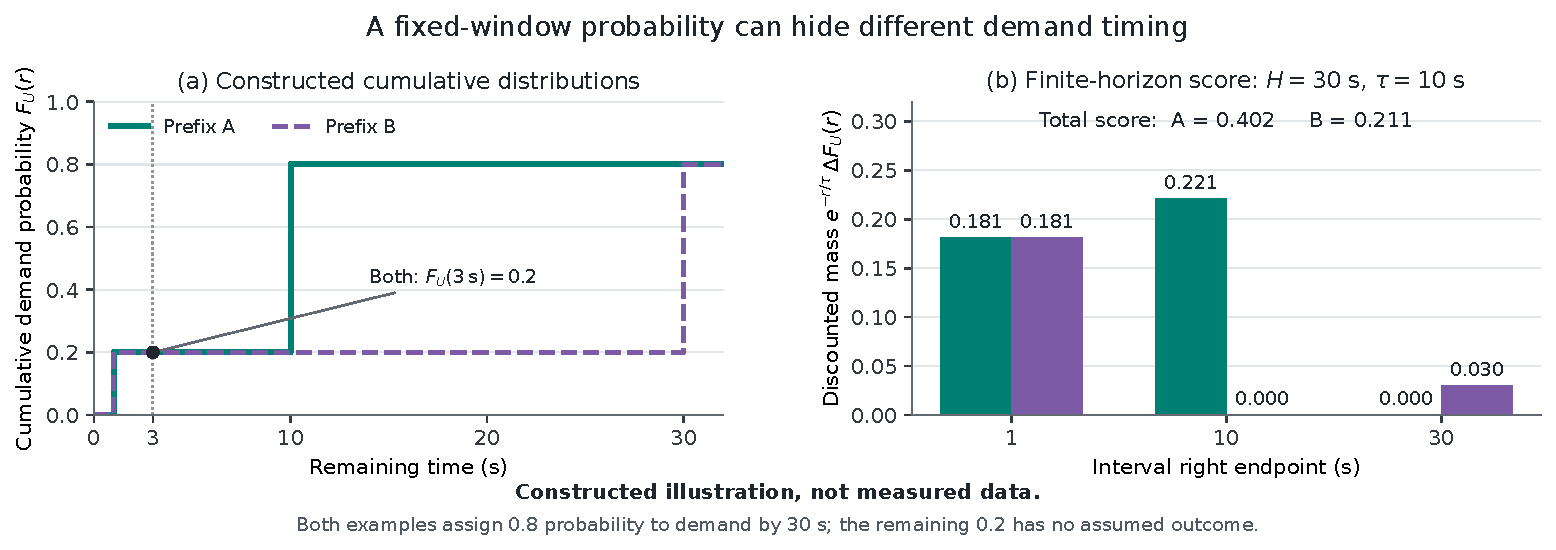
\includegraphics[width=0.95\linewidth,height=\textheight,keepaspectratio,alt={Constructed illustration, not measured data. A and B have equal three-second cumulative demand probability and equal demand mass through 30 seconds, but different temporal allocations and discounted scores. Unresolved mass is not reassigned to demand.}]{leasepath_iclr_v1_assets/figures/figure1_distribution_example.pdf}
\caption{Constructed illustration, not measured data. A and B have equal
three-second cumulative demand probability and equal demand mass through
30 seconds, but different temporal allocations and discounted scores.
Unresolved mass is not reassigned to
demand.}\label{fig:distribution-example}
\end{figure}

The score has simple interpretive properties. Right-endpoint discounting
lower-bounds the corresponding continuous discounted functional of the
same distribution; pointwise dominance of cumulative demand
probabilities on the grid preserves the discrete score ordering.
Appendix B gives these facts and a conditional perturbation bound. They
explain the proxy and do not establish optimal cache decisions.

\subsection{4.3 Pressure-triggered legal
eviction}\label{pressure-triggered-legal-eviction}

Algorithm 1 describes the main equal-cost policy. The controller fixes
one decision time for an admission and memoizes each encountered owner's
prediction. It removes one logical leaf at a time, recomputing feasible
leaves and live bindings. The completed deletion plan is then submitted
to the native backend; the implementation does not invoke a separate
native deletion after every logical comparison.

\Needspace{30\baselineskip}

\textbf{Algorithm 1: LeasePath admission and eviction.}

\begin{Shaded}
\begin{Highlighting}[]
\NormalTok{Input: compatible request prefix, resident tree, references,}
\NormalTok{       frozen predictor, admission timestamp t0}
\NormalTok{1. Validate ancestry, request size, and protected{-}capacity feasibility.}
\NormalTok{2. Protect active blocks and the current request\textquotesingle{}s prefix.}
\NormalTok{3. Initialize an owner memo using fixed t0, and an empty drop plan.}
\NormalTok{4. fallback \textless{}{-} false}
\NormalTok{5. While the request cannot fit within the persistent quota:}
\NormalTok{     Recompute unprotected leaves and reachable owner bindings.}
\NormalTok{     If unbound leaves exist:}
\NormalTok{         Choose one by (touched, {-}depth, key).}
\NormalTok{     Otherwise:}
\NormalTok{         Predict newly encountered owners once, using state at t0.}
\NormalTok{         If any required distribution score is unavailable:}
\NormalTok{             fallback \textless{}{-} true}
\NormalTok{         If fallback:}
\NormalTok{             Choose a leaf by the retired{-}first LRU ordering.}
\NormalTok{         Otherwise:}
\NormalTok{             Choose the minimum (V\_b, touched, {-}depth, key).}
\NormalTok{     Remove the leaf from the logical tree; append to drop plan.}
\NormalTok{6. Submit the drop plan to native KV storage; verify mappings/cells.}
\NormalTok{7. Call native generation, which checks native request bounds.}
\NormalTok{8. On normal model completion, release its context to idle.}
\NormalTok{   On abort, clean up unmaterialized suffix and active ownership.}
\end{Highlighting}
\end{Shaded}

Admission fails when protected active state makes the request
infeasible; the controller does not violate active-reference constraints
to force progress. The fixed timestamp is passed to the logical
controller at admission. Native generation bounds are checked when
generation is invoked, after the deletion plan has been applied; the
prototype does not guarantee that every backend rejection precedes all
cache changes. A missing or invalid distribution triggers LRU ordering
for the remainder of that admission. Previously selected actions are not
retroactively undone. Without capacity pressure, scoring is unnecessary.

The current implementation scans candidates and updates the logical
structure repeatedly. Its prediction memo reduces repeated calls within
an admission, but it does not provide a heap-based logarithmic eviction
algorithm. Scalability depends on the number of owners, candidate
leaves, and required removals, and needs measurement beyond the present
small setting.

\subsection{4.4 Support and fallback}\label{support-and-fallback}

The distribution score requires the horizon to coincide with an
available right endpoint and every interval through \(H\) to have at
least five training workflows in its global risk support. At the
30-second interval, the frozen training data provide only six workflows.
Passing the support gate therefore does not imply a reliable statistical
confidence bound.

Unseen tool, phase, or elapsed categories invoke the predictor's
training-global fallback; an unsupported compatibility class yields an
unsupported distribution. These are different from the controller
falling back to LRU because the common window is unavailable. Invalid
probability output is recorded as an error, not silently interpreted as
zero demand or retirement.

The fixed-window comparator checks support at its three-second output.
Its implementation does not impose the distribution policy's additional
five-workflow condition across the whole 30-second horizon. These
support rules must not be described as identical. No distribution
fallback was observed in the completed natural experiment, but
comparisons under support failure require separate analysis.

\subsection{4.5 Cost-weighted extension}\label{cost-weighted-extension}

We also implement a cost multiplier using an independently calibrated
prefill table. Let \(P_i\) be the currently observed, block-aligned
prefix length and \(\ell_i\) the continuously resident prefix length.
For 128-token blocks, the estimated marginal cost is

\[
\widehat C_{i,b}=\widehat T(P_i+1,\ell_i-128)
 -\widehat T(P_i+1,\ell_i),
\qquad
V_b^{\mathrm{cost}}=\frac{\max_{i\in\mathcal O_b}
 (\widehat C_{i,b}W_i)}{B_b}.
\]

The extra token satisfies the backend's requirement to leave an uncached
token in the calibration request; it is not a prediction of the future
suffix. The table uses exact supported grid points without interpolation
or extrapolation. Missing cost support switches the remaining admission
comparisons to equal cost, separately from distribution-to-LRU fallback.
Continuous resident length and marginal cost are updated after logical
removals.

This extension is an ablation, not part of the main successful
configuration. It underperforms equal-cost scoring in the current
experiment. A good fit on calibration prompts does not by itself
establish a good estimate of the cost of a future request containing new
tool output.

\subsection{4.6 Native realization}\label{native-realization}

The adapter executes real KV reference deletion and checks physical
token/cell mappings around requests. Shared payload is counted once, and
generated outputs and consumed tool feedback are linked to the event
stream. The backend preallocates its device KV buffer. Eviction frees
used cells and references for reuse within that allocation; it does not
shrink reserved CUDA memory. We distinguish the persistent payload
quota, used physical cells, and reserved device bytes. The logical
blocks should not be equated with the implementation of paged blocks in
another serving engine.

\section{5 Experimental Design}\label{experimental-design}

\subsection{5.1 Questions and evidence
units}\label{questions-and-evidence-units}

The completed experiments address whether a different functional of the
same predictor changes actual reuse and measured completion time,
whether the frozen predictor improves on empirical estimates, and
whether a marginal-cost multiplier helps. Independent-task
generalization, comparison with complete prior systems, broad cache
pressure, and full overhead amortization remain open.

Table 1 separates the data used for these questions. A parent task is
the grouping unit for prediction evaluation. The online experiment
repeats three known parents in four time cycles; it does not contain 48
independent task types.

\begin{longtable}[]{@{}
  >{\raggedright\arraybackslash}p{(\linewidth - 6\tabcolsep) * \real{0.2500}}
  >{\raggedleft\arraybackslash}p{(\linewidth - 6\tabcolsep) * \real{0.2500}}
  >{\raggedright\arraybackslash}p{(\linewidth - 6\tabcolsep) * \real{0.2500}}
  >{\raggedright\arraybackslash}p{(\linewidth - 6\tabcolsep) * \real{0.2500}}@{}}
\toprule\noalign{}
\begin{minipage}[b]{\linewidth}\raggedright
Evidence set
\end{minipage} & \begin{minipage}[b]{\linewidth}\raggedleft
Parent tasks
\end{minipage} & \begin{minipage}[b]{\linewidth}\raggedright
Episodes / snapshots
\end{minipage} & \begin{minipage}[b]{\linewidth}\raggedright
Role
\end{minipage} \\
\midrule\noalign{}
\endhead
\bottomrule\noalign{}
\endlastfoot
Current-server development collection & 50 & 150 / 347 & Data and
predictor development \\
Internal training subset & 40 & 119 / 275 & Frozen estimators \\
Internal evaluation subset & 10 & 31 / 72 & Same-source prediction
evaluation \\
Natural policy experiment & 3 known parents & 48 task executions, 16
batches & Four-policy comparison \\
\end{longtable}

Table 1: Completed evidence only. The 50-task collection has episode
outcomes \(U/D/C=100/50/0\); train and evaluation subsets have
\(79/40/0\) and \(21/10/0\), respectively. Online task executions and
prediction episodes are different units.

The development tasks are local data-analysis workloads spanning SQL,
machine learning, cleaning, statistics, time series, and numerical
analysis. They share authorship, libraries, and some data structures.
The collection initially succeeded on 49 of 50 parents; after retaining
the failed attempt and rerunning the complete 38-task extension batch,
the accepted collection contains 50 successful parents. The prediction
results therefore describe the accepted collection, not a 100\%
first-attempt success rate. Historical data from a different server and
earlier Codex/MBPP workflows are not merged into these counts.

\subsection{5.2 Prediction protocol}\label{prediction-protocol}

The 40/10 split was fixed by semantic strata and a hash-based ordering
with seed 23 before fitting. Entire parents, their episodes, and
snapshots remain together. All 50 tasks had already been inspected
during development, so the split is an internal holdout, not an
untouched final test. The estimators use training-only vocabularies and
support counts, with no parameter search, early stopping, or refit on
all 50 parents.

We report the parent-weighted cumulative three-class Brier score for
\((F_U,F_D,S)\); its range is 0--2, and lower is better. It is not
answer accuracy. The same snapshots and supported windows are used
across predictors. Appendix C specifies time bins and model settings.
The test snapshots contain no demand within 0.1 seconds, even though
that horizon was the original primary prediction metric. Longer,
decision-relevant horizons are therefore reported alongside it.

\subsection{5.3 Execution platform and controlled
comparisons}\label{execution-platform-and-controlled-comparisons}

The native backend serves Qwen2.5-Coder-32B-Instruct from an unquantized
F16 GGUF model with F16 KV storage, using llama.cpp/CUDA and three V100
GPUs with 32 GiB each. The model is split by layers across GPUs. The
physical context is 16,384 tokens. Each managed block holds 128 tokens
and represents 32 MiB of KV payload. The completed experiment uses 24
persistent blocks, equivalent to 3,072 tokens or 768 MiB of payload, and
2,048 tokens of transient headroom. Model requests run serially in FCFS
order; three sessions and their tools can overlap. Each tool uses one
numerical thread.

The four policies share inputs, model, execution protocol, native
controller, legal action space, unbound-state reclamation, tie-breaking,
resource settings, and auditing:

\begin{itemize}
\tightlist
\item
  \textbf{A, retired-first LRU:} reclaim unbound legal leaves first,
  then order live candidates by recency.
\item
  \textbf{B, fixed-window probability:} use \(F_U(3\,\mathrm{s})\) from
  the frozen GBDT, with equal costs.
\item
  \textbf{C, LeasePath equal cost:} use the same GBDT and \(W\) with
  \(H=30\) seconds and \(\tau=10\) seconds.
\item
  \textbf{D, LeasePath with cost:} multiply the same discounted mass by
  calibrated marginal cost.
\end{itemize}

The code identifier \nolinkurl{gbdt_point} refers to B, but we use
``fixed-window probability'' throughout the paper to avoid confusing it
with a time prediction. Conditional empirical prediction has been
evaluated offline; its online combination with the same distribution
controller remains a required comparator.

The online parents are logistic holdout evaluation, ridge
cross-validation, and temporal as-of matching. All three belong to the
previously viewed ten-parent internal evaluation subset. Each policy
executes one three-session batch in each of four cycles, using a
Williams order: A--B--D--C, B--C--A--D, C--D--B--A, and D--A--C--B.
Every policy occupies each position once, and each directed adjacent
pair appears once. This balances order in this small experiment; it does
not create additional independent workloads.

\subsection{5.4 Measurement, quality, and
interference}\label{measurement-quality-and-interference}

JCT is measured from common batch submission to independently validated
final answers as defined in Section 3.3. Cached tokens, actual prefill
tokens, prefill time, and controller measurements are aggregated per
three-session batch. JCT is averaged per task. Overlapping tool times
and aggregate model times cannot simply be added to reconstruct a task's
critical path.

All policies run real tools and consume their results in subsequent
actual prompts. Final acceptance checks the response schema, output
artifacts, task references, and feedback consumption. The completed
experiment contains 144 live generations and 13 native probes; a
separate traced diagnostic is excluded from natural timing. We report
all 48 task executions in the completed comparison, all of which pass
validation.

The server is shared. Fixed CPU affinity, numerical thread limits,
NUMA/THP controls, pinned model and dependency pages, and prospective
I/O and major-fault gates reduce specific interference sources. They do
not reserve CPU cores or memory bandwidth. A violation stops the attempt
and remains in the evidence; slow observations are not replaced based on
JCT. Natural timing excludes tracing, while audit work performed inside
the controller remains included.

We report cycle-paired differences descriptively. Four cycles and three
known parents do not support a population significance claim or a
reliable tail-latency estimate. A future analysis must freeze
repetitions, source-family weighting, and uncertainty estimation before
observing the final independent results.

\section{6 Results and Analysis}\label{results-and-analysis}

\subsection{6.1 Conditional empirical prediction is stronger on current
data}\label{conditional-empirical-prediction-is-stronger-on-current-data}

Table 2 shows that the conditional empirical estimator outperforms both
the global estimator and the frozen GBDT at every displayed window. At
three seconds, for example, its Brier score is 0.4677 versus 0.5227 for
GBDT. The result argues against treating model complexity as the
contribution: the online GBDT is a frozen candidate used to control
prediction information across policies, not the best predictor
established by this offline comparison.

\begin{longtable}[]{@{}rrrr@{}}
\toprule\noalign{}
Horizon & Global empirical & Conditional empirical & Frozen GBDT \\
\midrule\noalign{}
\endhead
\bottomrule\noalign{}
\endlastfoot
0.1 s & 0.4388 & \textbf{0.2976} & 0.3903 \\
1 s & 0.6682 & \textbf{0.4900} & 0.5791 \\
3 s & 0.5900 & \textbf{0.4677} & 0.5227 \\
10 s & 0.4977 & \textbf{0.3689} & 0.4297 \\
30 s & 0.4750 & \textbf{0.3423} & 0.3975 \\
\end{longtable}

Table 2: Parent-weighted cumulative Brier score on 72 snapshots from ten
internal evaluation parents. Lower is better; scores are squared errors,
not percentages. All displayed horizons use the same snapshots.

The 0.1-second result primarily distinguishes retirement from continued
waiting because no test snapshot has a demand within that horizon. The
longest test episode is approximately 52.4 seconds, with no test episode
reaching 60 seconds. The two parents with episodes at least 60 seconds
long are in training. The 600-second interval has no training risk
support and is excluded rather than filled using test outcomes. These
coverage limits prevent a claim of accurate long-tail demand prediction.

Single-call median prediction latency in the recorded CPU microbenchmark
is approximately 0.067 ms for global empirical estimation, 0.087 ms for
conditional empirical estimation, and 0.648 ms for GBDT. These figures
exclude full online state preparation and cache control. Whether the
stronger empirical estimator yields better online retention remains
unmeasured.

\subsection{6.2 Distribution scoring changes real reuse and
prefill}\label{distribution-scoring-changes-real-reuse-and-prefill}

Table 3 reports the completed natural comparison. Relative to A,
equal-cost distribution scoring C reuses 768 additional tokens per batch
and reduces executed prefill by the same number of tokens. Aggregate
prefill time falls from 10.7162 to 9.1516 seconds per batch, a reduction
of 1.5646 seconds or 14.600\%. Mean JCT falls from 52.8505 to 51.3025
seconds, a reduction of 1.5480 seconds or 2.929\%.

\begin{longtable}[]{@{}
  >{\raggedright\arraybackslash}p{(\linewidth - 10\tabcolsep) * \real{0.2400}}
  >{\raggedleft\arraybackslash}p{(\linewidth - 10\tabcolsep) * \real{0.1520}}
  >{\raggedleft\arraybackslash}p{(\linewidth - 10\tabcolsep) * \real{0.1520}}
  >{\raggedleft\arraybackslash}p{(\linewidth - 10\tabcolsep) * \real{0.1520}}
  >{\raggedleft\arraybackslash}p{(\linewidth - 10\tabcolsep) * \real{0.1520}}
  >{\raggedleft\arraybackslash}p{(\linewidth - 10\tabcolsep) * \real{0.1520}}@{}}
\toprule\noalign{}
\begin{minipage}[b]{\linewidth}\raggedright
Policy
\end{minipage} & \begin{minipage}[b]{\linewidth}\raggedleft
Cached tokens / batch
\end{minipage} & \begin{minipage}[b]{\linewidth}\raggedleft
Prefill tokens / batch
\end{minipage} & \begin{minipage}[b]{\linewidth}\raggedleft
Prefill s / batch
\end{minipage} & \begin{minipage}[b]{\linewidth}\raggedleft
JCT s / task
\end{minipage} & \begin{minipage}[b]{\linewidth}\raggedleft
JCT reduction vs A
\end{minipage} \\
\midrule\noalign{}
\endhead
\bottomrule\noalign{}
\endlastfoot
A: LRU & 7,424 & 7,130 & 10.7162 & 52.8505 & --- \\
B: \(F_U(3\,\mathrm{s})\) & 7,808 & 6,746 & 9.9087 & 52.2020 &
1.227\% \\
C: Distribution & \textbf{8,192} & \textbf{6,362} & \textbf{9.1516} &
\textbf{51.3025} & \textbf{2.929\%} \\
D: Distribution × cost & 7,808 & 6,746 & 10.0575 & 51.9522 & 1.700\% \\
\end{longtable}

Table 3: Preliminary natural execution, 24 blocks and three concurrent
sessions. A is retired-first LRU; B--D share the same frozen GBDT. Each
policy has four batches and twelve task executions from the same three
known parents; 48/48 executions validate. Relative changes use unrounded
aggregates. The setting is shared-server development evaluation.

Compared with B, C reuses 384 additional tokens per batch, reduces
prefill time by 0.7571 seconds, and reduces mean JCT by 0.8995 seconds
or 1.723\%. Because B and C use the same frozen predictor, this
comparison associates the changed score functional with a different
physical reuse outcome in this workload. It does not establish that the
frozen distribution is well calibrated or that a complete external
system would be slower.

\begin{figure}
\centering
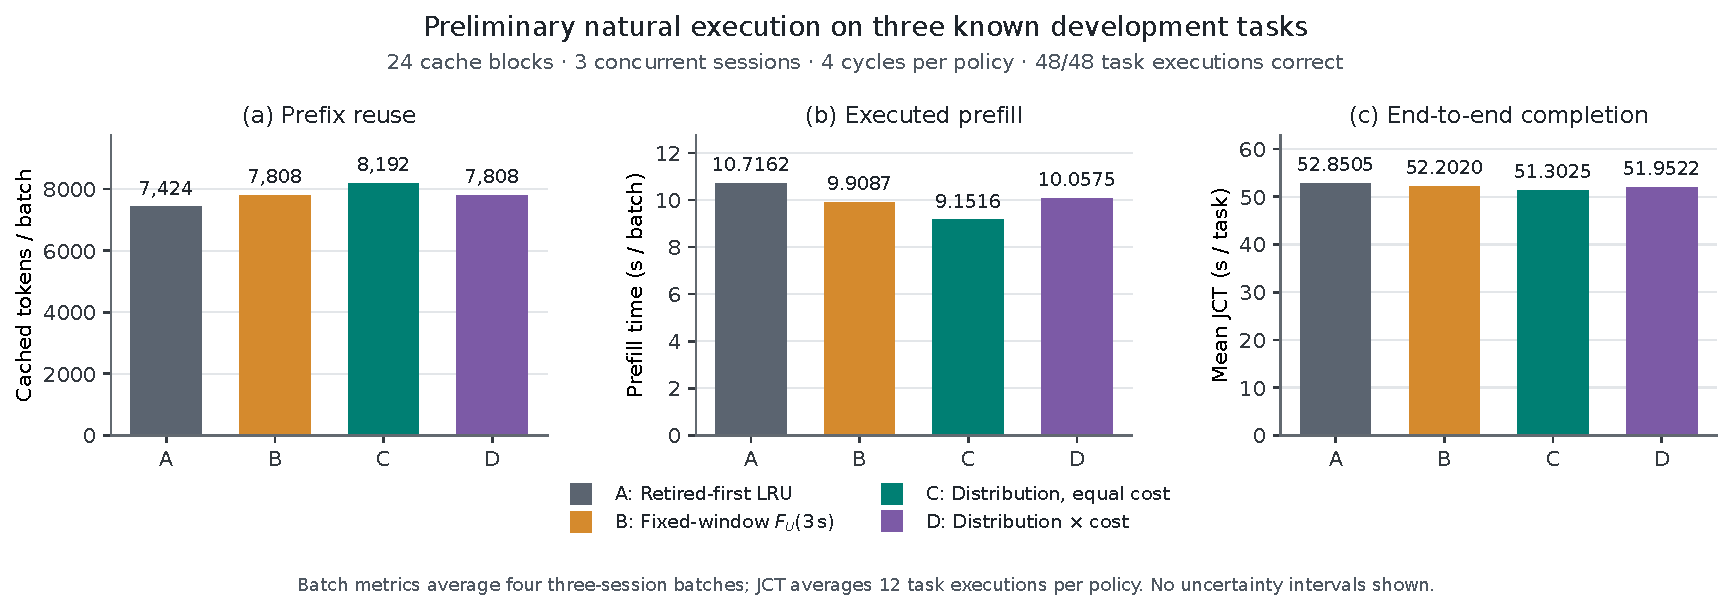
\includegraphics[width=1\linewidth,height=\textheight,keepaspectratio,alt={Completed preliminary comparison. Bars start at zero and show separate measurement levels: cached tokens and prefill seconds per three-session batch, and JCT seconds per task. Four repeated cycles per policy cover three known development tasks; no confidence intervals are inferred from these aggregates.}]{leasepath_iclr_v1_assets/figures/figure2_preliminary_results.pdf}
\caption{Completed preliminary comparison. Bars start at zero and show
separate measurement levels: cached tokens and prefill seconds per
three-session batch, and JCT seconds per task. Four repeated cycles per
policy cover three known development tasks; no confidence intervals are
inferred from these aggregates.}\label{fig:preliminary-results}
\end{figure}

Both C--A and C--B mean-JCT differences are negative in all four cycles
(Figure 3). C--A ranges from −1.999 to −1.053 seconds; C--B ranges from
−1.621 to −0.423 seconds. The consistency is descriptive evidence within
these cycles, not a statistical generalization claim. Mean batch
makespan is 68.2116 seconds for A, 67.6207 for B, 66.4738 for C, and
67.1262 for D.

\begin{figure}
\centering
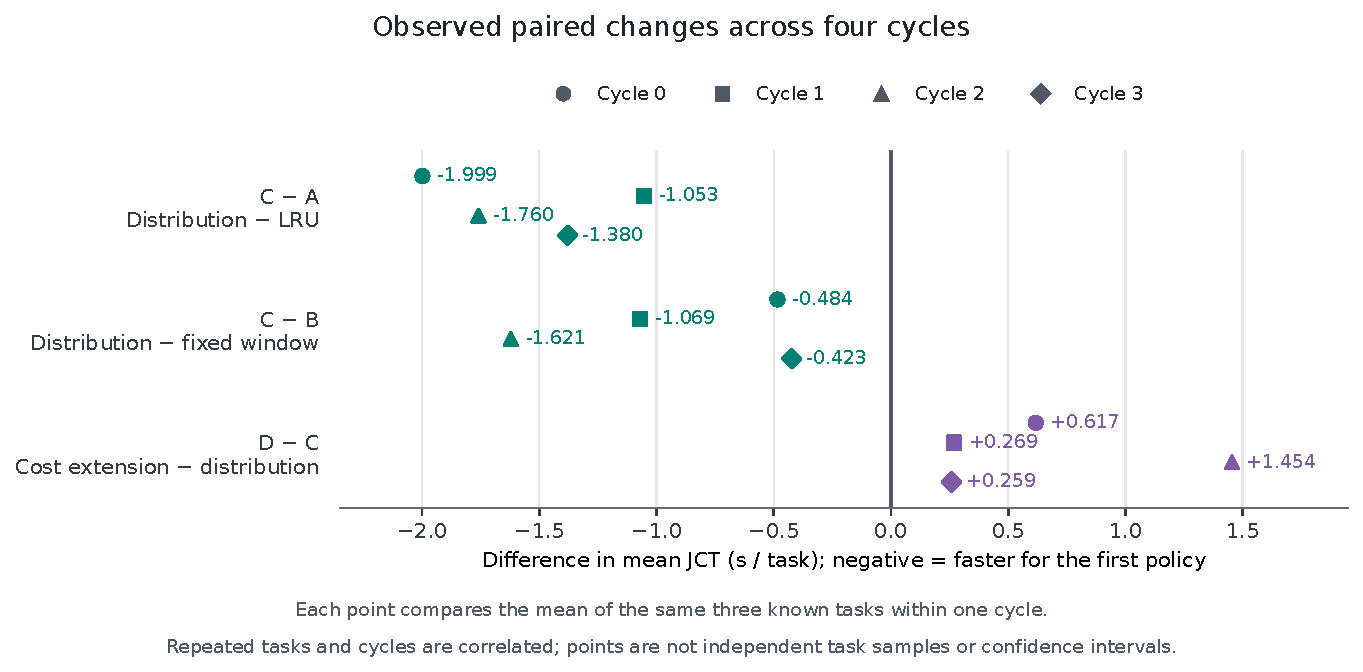
\includegraphics[width=0.95\linewidth,height=\textheight,keepaspectratio,alt={Within-cycle differences in mean JCT: negative C−A and C−B values favor equal-cost distribution scoring; positive D−C values favor equal cost over the cost extension. Each point is one repeated time cycle on the same three tasks, not an independent task-family sample.}]{leasepath_iclr_v1_assets/figures/figure3_paired_cycles.pdf}
\caption{Within-cycle differences in mean JCT: negative C−A and C−B
values favor equal-cost distribution scoring; positive D−C values favor
equal cost over the cost extension. Each point is one repeated time
cycle on the same three tasks, not an independent task-family
sample.}\label{fig:paired-cycles}
\end{figure}

\subsection{6.3 A calibrated cost multiplier does not improve the
result}\label{a-calibrated-cost-multiplier-does-not-improve-the-result}

Adding marginal cost worsens mean JCT by 0.6497 seconds, or 1.266\%,
relative to equal-cost distribution scoring. D is slower than C in all
four cycles and reuses 384 fewer tokens per batch. This occurs despite
an independent 79-point calibration validation with mean absolute error
of 2.607 ms on its fixed prompt/length grid. There is no observed cost
or distribution fallback in these runs.

The request-level evidence helps identify the mismatch without resolving
its full cause. Relative to C, D loses 256 cached tokens on logistic
evaluation and 256 on temporal matching, while gaining 128 on ridge
validation. C and D have identical corresponding input and output
tokens. For one first-cycle logistic continuation, the actual request
has 1,777 tokens, while the previously observed block-aligned prefix has
1,536. C reuses 1,152 tokens and D reuses 896, with measured prefill of
0.87787 and 1.39069 seconds, respectively. The future 241-token
extension is used only in this post hoc diagnosis; it was not available
to the policy.

The cost table is calibrated on the observed prefix plus one token,
whereas later prompts include tool results and protocol text. Native
512-token batch boundaries and prefix dependencies can further change
the marginal value of a leaf. These are plausible explanations for the
proxy's failure, not independently isolated causal effects. The result
supports keeping equal cost as the current primary configuration, while
leaving the value of better causal cost models open.

\subsection{6.4 Completion-time attribution and controller
overhead}\label{completion-time-attribution-and-controller-overhead}

The natural experiment includes controller work, but it does not isolate
all causes of the observed JCT differences. Corresponding input tokens
are identical across policies. A and B average 651 generated tokens per
batch; C and D average 650. Thus comparisons between these groups
include a small output-length difference. Tool wall times also vary; for
example, mean logistic tool time is 9.3854 seconds under C and 10.5710
seconds under D. Even C--D, with matched input and output tokens, cannot
attribute its entire JCT difference to caching.

\begin{longtable}[]{@{}
  >{\raggedright\arraybackslash}p{(\linewidth - 6\tabcolsep) * \real{0.2500}}
  >{\raggedleft\arraybackslash}p{(\linewidth - 6\tabcolsep) * \real{0.2500}}
  >{\raggedleft\arraybackslash}p{(\linewidth - 6\tabcolsep) * \real{0.2500}}
  >{\raggedleft\arraybackslash}p{(\linewidth - 6\tabcolsep) * \real{0.2500}}@{}}
\toprule\noalign{}
\begin{minipage}[b]{\linewidth}\raggedright
Policy
\end{minipage} & \begin{minipage}[b]{\linewidth}\raggedleft
Prediction ms / batch
\end{minipage} & \begin{minipage}[b]{\linewidth}\raggedleft
Logical admission + shadows ms / batch
\end{minipage} & \begin{minipage}[b]{\linewidth}\raggedleft
Controller prepare ms / batch
\end{minipage} \\
\midrule\noalign{}
\endhead
\bottomrule\noalign{}
\endlastfoot
A & 8.663 & 34.858 & 177.519 \\
B & 8.807 & 39.472 & 176.460 \\
C & 9.591 & 33.525 & 252.049 \\
D & 10.478 & 36.846 & 179.393 \\
\end{longtable}

Table 4: Observed instrumentation categories, averaged over four
three-session batches per policy. Categories overlap and must not be
added. Controller preparation includes native inspection, deletion, and
mapping work; it is not a direct timing of score integration alone.

LRU also incurs shadow-prediction auditing in this experiment.
Therefore, the observed improvement over A is a net difference between
these instrumented configurations, not an established net gain over a
minimal LRU without shadow computation. Initialization and
page-residency preparation are outside the JCT window and have not been
amortized over workload size.

Physical and protocol audits support the validity of the measurement
chain: 157/157 requests map to the ledger, all 48 final answers
validate, and 96 real tool results are consumed by later requests. All
16 batches pass the specified zero-increment parent read-byte,
major-fault, and block-input gates. These checks cannot prove absence of
shared-host noise. Recorded CPU pressure spans 0.393\%--60.482\%, and
I/O pressure spans 1.094\%--5.777\%. The conclusions therefore remain
paired observations under this shared-server configuration.

\subsection{6.5 Independent evaluation remains
open}\label{independent-evaluation-remains-open}

No independent main-result table is filled in this version. The
outline's evidence cutoff precedes new natural results from the
registered \(24/32/64\)-block by \(3/6/10\)-session matrix. Its future
results must be reported separately from the older 24-block experiment
because the resource configuration changes. The registered matrix uses
three policies and all six policy permutations, totaling eighteen
batches per cell; it is not the four-policy Williams experiment above.

Twelve local candidate instances have been prepared with a
six-development/six-held-out source-family split and exclusion of the
old 50 parents. They are small authored protocol instances, not
representative samples imported from an external benchmark.
Source-family naming alone does not establish independent authorship or
problem structure. Their manifest and reference checks are preparation
evidence, not proof that new model-driven iterative loops have passed.
This draft does not use their held-out answers or outcomes to select the
method.

The main unresolved comparisons are conditional empirical distributions
with the same controller, conditional-mean or quantile ordering derived
under a clearly stated support window, faithful CacheWise and TTL
comparators, and lifecycle-matched baselines. Workload variation must
include low pressure, meaningful competition, overload, prefix lengths,
sharing, and genuine tool-time variation. Independent results may narrow
or reverse the preliminary finding.

\section{7 Limitations and Responsible
Evaluation}\label{limitations-and-responsible-evaluation}

The current data mainly cover short local data-analysis trajectories
with simple termination. All observed episode outcomes are demand or
explicit retirement; there is no natural censoring. Complex
cancellation, version replacement, open-ended coding, network tools,
human waiting, and broad branching behavior remain underrepresented.
More snapshots from the same trajectory would not fix this lack of
independent coverage.

The predictor uses coarse features. Elapsed buckets stop at one second,
so sessions with the same tool and phase can receive unchanged
predictions throughout much longer waits. Repeated calls do not create
fine-grained adaptation. Tail support is sparse, queue features are
absent, and lookup-time distributions can shift when policy-induced
service times change. The scoring horizon, discount, maximum-owner
aggregation, and leaf-greedy procedure are engineering choices rather
than an optimal control solution.

The system evidence covers one model, one native adapter, layer
splitting over three GPUs, a fixed 16K context, and serial FCFS model
service. It does not establish behavior under production continuous
batching or a different offload hierarchy. The few-percent JCT
observation requires independent repeated measurements, matched quality
reporting, stronger baselines, and comparison without unnecessary
auditing overhead before a broader performance claim is warranted.

Tool execution retains its existing permission and resource boundaries.
A cache policy must not alter those boundaries to improve timing.
Released traces require review for sensitive inputs, code, and tool
output, together with source and redistribution permissions.
Reproducibility should retain failed attempts and distinguish
constructed mechanism examples, fixed-state diagnostics, and natural
execution. Public tool logs lacking actual compatible lookup events
cannot be relabeled as ground-truth demand data.

\section{8 Conclusion}\label{conclusion}

LeasePath studies the use of remaining-time distributions of legal
prefix demand for KV retention in tool-augmented agents. It maps
finite-horizon discounted probability mass to a feasible sequence of
prefix-leaf removals, then executes and audits the resulting native KV
actions. In a restricted three-task development experiment, this mapping
increases actual reuse and reduces measured prefill and mean
validated-answer completion time relative to two internal baselines.
Conditional empirical prediction is stronger than the frozen GBDT
offline, and a calibrated cost extension does not improve the online
result. The present evidence supports investigating the
demand-to-decision connection while leaving independent generalization,
complete-system comparisons, and broader net benefit unresolved.

\clearpage

\section{References}\label{references}

Abhyankar, Reyna, Zijian He, Vikranth Srivatsa, Hao Zhang, and Yiying
Zhang. 2024. \emph{InferCept: Efficient Intercept Support for Augmented
Large Language Model Inference}. arXiv:2402.01869v2.
\href{https://arxiv.org/abs/2402.01869v2}{Specified version}.

Fu, Kaihua, et al.~2026. \emph{Capture the lifecycle: KV Cache
management in ReAct Agents with KVTether}. arXiv:2609.39819v1.
\href{https://arxiv.org/abs/2609.39819v1}{Specified version}.

Lee, Changhee, William R. Zame, Jinsung Yoon, and Mihaela van der
Schaar. 2018. \emph{DeepHit: A Deep Learning Approach to Survival
Analysis with Competing Risks}. AAAI.
\href{https://cdn.aaai.org/ojs/11842/11842-13-15370-1-2-20201228.pdf}{Official
paper}.

Li, Hanchen, et al.~2025. \emph{Continuum: Efficient and Robust
Multi-Turn LLM Agent Scheduling with KV Cache Time-to-Live}.
arXiv:2511.02230. Version consulted: v7, September 8, 2026.
\href{https://arxiv.org/abs/2511.02230v7}{Specified version}.

Pan, Zaifeng, et al.~2025. \emph{KVFlow: Efficient Prefix Caching for
Accelerating LLM-Based Multi-Agent Workflows}. arXiv:2507.07400v1.
\href{https://arxiv.org/abs/2507.07400v1}{Specified version}.

Song, Berger, Li, and Lloyd. 2020. \emph{Learning Relaxed Belady for
Content Distribution Network Caching}. NSDI.
\href{https://www.usenix.org/conference/nsdi20/presentation/song}{Original
publication page}. \textbf{Bibliographic recheck pending:} the official
site returned HTTP 403 during preparation of v1; this entry retains the
earlier local survey's record.

Tiwari, Shubham, Tapan Chugh, Nash Rickert, Simon Peter, Ratul Mahajan,
and Haiying Shen. 2026. \emph{CacheWise: Understanding Workloads and
Optimizing KVCache Management for Efficiently Serving LLM Coding
Agents}. arXiv:2606.16824v1.
\href{https://arxiv.org/abs/2606.16824v1}{Specified version}.

Zheng, Haoyu, et al.~2026. \emph{Efficient Serving for Dynamic Agent
Workflows with Prediction-based KV-Cache Management}.
arXiv:2605.06472v1. \href{https://arxiv.org/abs/2605.06472v1}{Specified
version}.

\clearpage

\section{Appendix A. Event and measurement
contract}\label{appendix-a.-event-and-measurement-contract}

The idle episode begins at \(t_{\mathrm{idle}}\), while a prediction
snapshot is taken later at \(t\). Elapsed idle time is
\(t-t_{\mathrm{idle}}\) and the label is the remaining time from \(t\).
These quantities must not be interchanged. Features are reconstructed
only from events observed by \(t\); fields such as the first future
lookup identifier and future compatible request tokens belong
exclusively to labeling and audit data.

The first compatible lookup closes the episode with \(U\), regardless of
whether its KV is still physically resident. Explicit retirement closes
it with \(D\). An incompatible lookup alone does not demonstrate
permanent nonreuse. At equal timestamps, the recorded event sequence
chooses the first endpoint: a demand recorded before observation end
remains an observed demand. Censoring at an interval endpoint permits
the completed survival interval to be labeled waiting; censoring inside
an interval masks that partial interval. No later intervals are
generated.

This contract depends on complete collection and correct relationship
declarations. Validating a submitted event stream cannot prove that the
collector recorded every real lookup. It also cannot prove that a
claimed retirement was semantically warranted. Coverage and collection
audits are therefore separate from schema checks.

In the completed natural runner, the common submission timestamp is
taken after the engine is cleared and before per-task preparation. Each
owner's recorded submission is this same timestamp. Final validation
precedes the recorded completion timestamp, while context retirement
follows it. The field \nolinkurl{jct_to_validated_answer_s} is the
difference. This precise endpoint replaces the outline's provisional
``admission-to-answer'' terminology.

\section{Appendix B. Elementary properties of the retention
score}\label{appendix-b.-elementary-properties-of-the-retention-score}

The following statements concern a fixed snapshot and a given valid
competing-risk distribution, not the quality of its estimate. Let
\(R\in(0,\infty]\) and assume \(F_U(0)=0\). Demand mass can be
defective: neither eventual demand nor eventual resolution is required.
Fix \(0=r_0<\cdots<r_m=H\), \(\tau>0\), and \(w_k=e^{-r_k/\tau}\). Write
\(\Delta F_U(k)=F_U(r_k)-F_U(r_{k-1})\).

\subsection{B.1 Discretization and
truncation}\label{b.1-discretization-and-truncation}

Define the continuous discounted functional

\[
J_H=\int_{(0,H]}e^{-r/\tau}\,dF_U(r),
\qquad W=\sum_{k=1}^{m}w_k\Delta F_U(k).
\]

Because the discount decreases within each interval,

\[
0\le J_H-W\le D_{\mathrm{grid}}
=\sum_{k=1}^{m}(e^{-r_{k-1}/\tau}-e^{-r_k/\tau})\Delta F_U(k).
\]

\textbf{Proof.} On \((r_{k-1},r_k]\), the integrand lies between the two
endpoint weights. Integrate both inequalities against the nonnegative
mass of that interval and sum. Mass exactly at a right endpoint belongs
to that interval; no zero-time atom is omitted under the stated
assumption.

For any extension beyond \(H\) consistent with the same first-event
\(U/D\) distribution,

\[
0\le J_\infty-J_H\le e^{-H/\tau}S(H),
\qquad
0\le J_\infty-W\le D_{\mathrm{grid}}+e^{-H/\tau}S(H).
\]

\textbf{Proof.} First demand after \(H\) has probability at most the
unresolved mass \(S(H)\), and its discount is at most \(e^{-H/\tau}\).
Demand after retirement belongs to another relationship and is not part
of this tail. If applied to a predicted distribution, this bound
concerns its own possible extension; predicted survival is not a
confidence bound for the true unknown tail.

\subsection{B.2 Cumulative-incidence
dominance}\label{b.2-cumulative-incidence-dominance}

Summation by parts gives

\[
W=w_mF_U(r_m)+\sum_{k=1}^{m-1}(w_k-w_{k+1})F_U(r_k).
\]

All coefficients are nonnegative. Therefore, if
\(F_{U,A}(r_k)\ge F_{U,B}(r_k)\) at every common endpoint, then
\(W_A\ge W_B\). This result does not require equal total demand
probability. It applies to the discrete score; endpoint dominance alone
does not compare the continuous functionals when event locations within
intervals differ. Dominance of time conditioned on eventual demand is
also insufficient when eventual demand probabilities differ.

\subsection{B.3 Perturbations and conditional ordering
stability}\label{b.3-perturbations-and-conditional-ordering-stability}

If two valid cumulative incidence estimates satisfy

\[
\max_k|\widehat F_U(r_k)-F_U(r_k)|\le\epsilon,
\]

the preceding identity and the triangle inequality imply

\[
|\widehat W-W|\le
\left[w_m+\sum_{k=1}^{m-1}(w_k-w_{k+1})\right]\epsilon
=w_1\epsilon.
\]

For a fixed nonempty owner set and positive block size, the maximum
aggregation is nonexpansive:

\[
|\widehat V_b-V_b|\le B_b^{-1}
\max_{i\in\mathcal O_b}|\widehat W_i-W_i|.
\]

If two candidates have error bounds \(\eta_a,\eta_b\) and their true
proxy gap obeys \(V_a-V_b>\eta_a+\eta_b\), their estimated order is
preserved. Equality may permit a tie. No empirical uniform \(\epsilon\)
is established by this draft's Brier results. The argument assumes fixed
feasible candidates, owner sets, costs, and bytes, and does not cover
fallback, later tree changes, or policy-induced distribution shift. It
is not an eviction-accuracy or JCT guarantee.

\section{Appendix C. Predictor and implementation
settings}\label{appendix-c.-predictor-and-implementation-settings}

The remaining-time boundaries, in seconds, are

\[
(0.01,0.03,0.1,0.3,1,3,10,30,60,120,300,600).
\]

Elapsed-time bucket boundaries are \((0.03,0.1,0.3,1)\) seconds.
Conditional empirical groups require at least three training workflows
and use prior weight one for shrinkage. The distribution controller's
five-workflow support requirement is a separate setting.

The LightGBM configuration uses 40 boosting iterations, learning rate
0.05, maximum depth two, at most four leaves, minimum leaf sample count
20, L1 penalty 0.1, and L2 penalty 10. Training produces 1,552
risk-interval rows and 120 trees, with at most three leaves actually
used. Input feature vocabularies, global support, and fitted
distributions derive only from the 40-parent training subset. No new
feature selection or model fitting is performed for this manuscript.

The main policy fixes \(H=30\) seconds, \(\tau=10\) seconds, 128 tokens
per block, 33,554,432 payload bytes per block, equal costs, and
maximum-owner aggregation. The predictor identity and implementation
hashes are recorded in the frozen baseline configuration. Adaptive
discount selection, prefetching, offload, request reordering, and online
retraining are not components of the measured configuration.

For reproducibility, the F16 model SHA256 in the natural-run
configuration is
\nolinkurl{0c2f9e4daac78e72b24f7c054416232a523f0fd2aeb37653747d3c21f7dca078};
the frozen predictor SHA256 is
\nolinkurl{283b3c829a48460360ccf6a1ac311e2e7989a90d74d2338e15e25b08f7e78c5c}.
Backend, CUDA, GPU, runtime, and cost-table identities should be
recovered from the archived run manifests rather than inferred from the
manuscript's current checkout. The outline and writing-time code audit
use checkout \nolinkurl{096d6c7}; the accepted policy freeze records
baseline commit \nolinkurl{284b5b634bb82bce1fa61e2b29f1d28c61da019d}.
Neither is a replacement for per-run provenance.

\section{Appendix D. Additional completed
measurements}\label{appendix-d.-additional-completed-measurements}

\begin{longtable}[]{@{}
  >{\raggedright\arraybackslash}p{(\linewidth - 8\tabcolsep) * \real{0.2000}}
  >{\raggedleft\arraybackslash}p{(\linewidth - 8\tabcolsep) * \real{0.2000}}
  >{\raggedleft\arraybackslash}p{(\linewidth - 8\tabcolsep) * \real{0.2000}}
  >{\raggedleft\arraybackslash}p{(\linewidth - 8\tabcolsep) * \real{0.2000}}
  >{\raggedleft\arraybackslash}p{(\linewidth - 8\tabcolsep) * \real{0.2000}}@{}}
\toprule\noalign{}
\begin{minipage}[b]{\linewidth}\raggedright
Difference in mean JCT, seconds
\end{minipage} & \begin{minipage}[b]{\linewidth}\raggedleft
Cycle 0
\end{minipage} & \begin{minipage}[b]{\linewidth}\raggedleft
Cycle 1
\end{minipage} & \begin{minipage}[b]{\linewidth}\raggedleft
Cycle 2
\end{minipage} & \begin{minipage}[b]{\linewidth}\raggedleft
Cycle 3
\end{minipage} \\
\midrule\noalign{}
\endhead
\bottomrule\noalign{}
\endlastfoot
C − A & −1.998932 & −1.053428 & −1.759916 & −1.379614 \\
C − B & −0.484385 & −1.069419 & −1.621289 & −0.423087 \\
D − C & +0.617347 & +0.268583 & +1.454166 & +0.258732 \\
\end{longtable}

Table 5: Descriptive cycle-paired differences underlying Figure 3. Each
value averages the same three task types within one policy batch. The
cycles retain repeated-task dependence.

\begin{longtable}[]{@{}
  >{\raggedright\arraybackslash}p{(\linewidth - 8\tabcolsep) * \real{0.2000}}
  >{\raggedleft\arraybackslash}p{(\linewidth - 8\tabcolsep) * \real{0.2000}}
  >{\raggedleft\arraybackslash}p{(\linewidth - 8\tabcolsep) * \real{0.2000}}
  >{\raggedleft\arraybackslash}p{(\linewidth - 8\tabcolsep) * \real{0.2000}}
  >{\raggedleft\arraybackslash}p{(\linewidth - 8\tabcolsep) * \real{0.2000}}@{}}
\toprule\noalign{}
\begin{minipage}[b]{\linewidth}\raggedright
Policy
\end{minipage} & \begin{minipage}[b]{\linewidth}\raggedleft
Decode s / batch
\end{minipage} & \begin{minipage}[b]{\linewidth}\raggedleft
Logistic tool s
\end{minipage} & \begin{minipage}[b]{\linewidth}\raggedleft
Ridge tool s
\end{minipage} & \begin{minipage}[b]{\linewidth}\raggedleft
Temporal tool s
\end{minipage} \\
\midrule\noalign{}
\endhead
\bottomrule\noalign{}
\endlastfoot
A & 53.4469 & 9.9869 & 18.7593 & 5.5644 \\
B & 53.3942 & 9.4514 & 18.9837 & 5.1240 \\
C & 53.2491 & 9.3854 & 19.1502 & 5.3735 \\
D & 53.2813 & 10.5710 & 18.8187 & 5.1952 \\
\end{longtable}

Table 6: Observed decode and tool wall times. Tool computations overlap
with other sessions. These values cannot be summed with prefill to
recover average task JCT.

The separate cost validation uses 79 points from block-aligned prefix
lengths 1,152, 1,280, 1,536, 1,664, 1,792, and 1,920 tokens and their
legal cached lengths. Calibration requests contain one additional
uncached token. Mean absolute error is 2.607 ms, approximately 0.2465\%
of mean calibration prefill time. The median positive marginal block
cost is 92.991 ms. These measurements characterize the calibration grid,
not unknown future tool suffixes.

All recorded natural comparison batches are retained. Earlier failed
preparations, traced diagnostics, and historical experiments remain
separate artifacts and are not inserted into the completed comparison's
mean. In particular, an instrumented diagnostic that validates physical
actions is not an additional natural performance replication.

\section{Appendix E. Evaluation required for broader
claims}\label{appendix-e.-evaluation-required-for-broader-claims}

The following work is unfinished in this version. This appendix records
research requirements, not changes to any running or frozen experiment.

\textbf{Pressure and independent workloads.} Complete the registered
capacity/concurrency evaluation, retaining failed cells and negative
gains. Report its new resource configuration separately. Validate new
development instances through actual model output, real tool parameters,
execution, feedback consumption, subsequent model decisions, and
independent final acceptance before freezing the independent evaluation.
A successful one-pass answer remains a success but should not be counted
as iterative revision.

\textbf{Predictor and decision-function separation.} Cross empirical and
learned predictors with fixed-window, discounted, and supported
mean/quantile scores under a common information set. A mean derived only
within a finite window must be described as restricted or truncated.
Faithful external comparisons need to disclose extra features,
scheduling, prefetching, storage tiers, and reproduction differences.
Fixed-state replay may explain why actions differ, while natural
execution supplies JCT.

\textbf{Mechanism and failure boundaries.} Record candidate sets,
protection, support, score differences, actual deletion, and subsequent
executed prefill. Vary prefix length, sharing, real tool-time
distributions, and cache pressure. Include no-pressure and retired-only
comparisons to distinguish distribution value from lifecycle
reclamation. Test the observed-prefix cost proxy separately from future
suffix effects and native batch boundaries.

\textbf{Uncertainty and total cost.} Freeze the main comparison,
aggregation weights, repeated time blocks, and source-family-aware
interval estimation before independent results are viewed. Preserve
correlations among snapshots, episodes, parents, and repeated time
blocks. Report quality and time for all attempts rather than only
successful ones. Any budget-penalized endpoint for failure must be
defined prospectively and kept distinct from actual failed-run duration.
Compare versions with matched necessary auditing and report
initialization separately from prepared-service JCT, including
amortization where appropriate.

\textbf{Data coverage.} Review source and near-duplicate independence,
tool and lifecycle coverage, missing-event semantics, and redistribution
rights. The current twelve-instance preparation is a pilot scale. More
independently sourced tasks and measured variance are needed to choose a
defensible evaluation size. Synthetic waits and repeated small
computation should not be presented as representative long-running
tools.

\section{Appendix F. Reproducibility and release
scope}\label{appendix-f.-reproducibility-and-release-scope}

The reproducibility package should preserve fixed task manifests,
grouped splits, input and reference hashes, prediction models, per-run
backend identities, successful and failed attempt ledgers, event
schemas, native audit records, raw timing, and resource gates. Audit
code should make it possible to follow a demand label to its lookup, a
cache action to its physical mapping, and a tool result to the
subsequent prompt that consumed it.

This draft adds no new training or runtime experiment. Its figures are
generated from the existing natural-comparison JSON and the explicitly
constructed example. The figure script and provenance hashes are
included with the manuscript. The scalar tables use the existing reports
and machine summaries, with relative changes computed from unrounded
aggregates.

The available local artifacts include private runtime paths and
source-dependent material. A public package requires path restoration
instructions, dependency version records, and a review of what may be
redistributed. Keeping an artifact locally does not establish permission
to publish third-party data or model files.

\section{Appendix G. Evidence index and reference
status}\label{appendix-g.-evidence-index-and-reference-status}

Paths below are relative to the repository containing this manuscript.
They identify audit inputs rather than new results.

\begin{itemize}
\tightlist
\item
  \textbf{Collection and labels:}
  \nolinkurl{reports/extension50_collection_2026-11-07.md} and
  \nolinkurl{results/migration/extension50_2026-11-07/fifty-parent-dataset-card.json}
  support Table 1 and the accepted-collection counts. The report retains
  first-attempt and rerun distinctions.
\item
  \textbf{Offline prediction:}
  \nolinkurl{reports/qwen50_prediction_holdout_2026-11-08.md} and
  \nolinkurl{results/prediction/qwen50_holdout_2026-11-08/} support
  Table 2, split construction, predictor settings, and coverage
  restrictions.
\item
  \textbf{Natural comparison:}
  \nolinkurl{reports/kv_distribution_natural_2026-11-09.md} and
  \nolinkurl{results/cache_policy/kv_distribution_natural_2026-11-09/natural-comparison.json}
  support Tables 3--6 and Figures 2--3. Task-specific request deltas are
  retained in the same result directory.
\item
  \textbf{Calibration:}
  \nolinkurl{reports/kv_distribution_v1_2026-11-09.md} and its linked
  calibration artifacts support the cost-grid validation.
\item
  \textbf{Frozen method:}
  \nolinkurl{configs/baselines/kv_equal_cost_distribution_v1.json},
  \nolinkurl{src/leasepath/distribution_cache.py}, and
  \nolinkurl{src/leasepath/qwen_cache_backend.py} support the score,
  support rules, logical removal sequence, and batched native deletion.
\item
  \textbf{Endpoint:}
  \nolinkurl{scripts/qwen_cache_resident_tree_batch.py} supports the
  shared submission timestamp and validation boundary.
  \nolinkurl{configs/prediction/qwen_distribution_natural_2026-11-09.json}
  records the measured protocol and resource settings.
\item
  \textbf{Event semantics:} \nolinkurl{docs/prediction_contract.md}, the
  current exporters, and the frozen method sources distinguish event
  definitions from historically available features.
\item
  \textbf{Prepared future evaluation:}
  \nolinkurl{docs/pressure_and_independent_agent_next_stage_2026-11-10.md}
  and the candidate manifest/family review linked by the outline
  document preparation status only. Their existence is not an evaluation
  result.
\end{itemize}

During preparation of v1, the specified arXiv versions of CacheWise,
Continuum, InferCept, KVFlow, PBKV, and KVTether were checked against
their metadata and relevant method text. DeepHit was checked against the
official AAAI PDF. The official LRB publication page and PDF were
inaccessible with HTTP 403, so its earlier local-survey entry remains
marked for recheck. Abbreviated author lists should be expanded and all
references checked against the eventual conference bibliography
requirements. No arXiv entry is asserted here to be a published
conference paper merely because it has an arXiv record.

\end{document}
